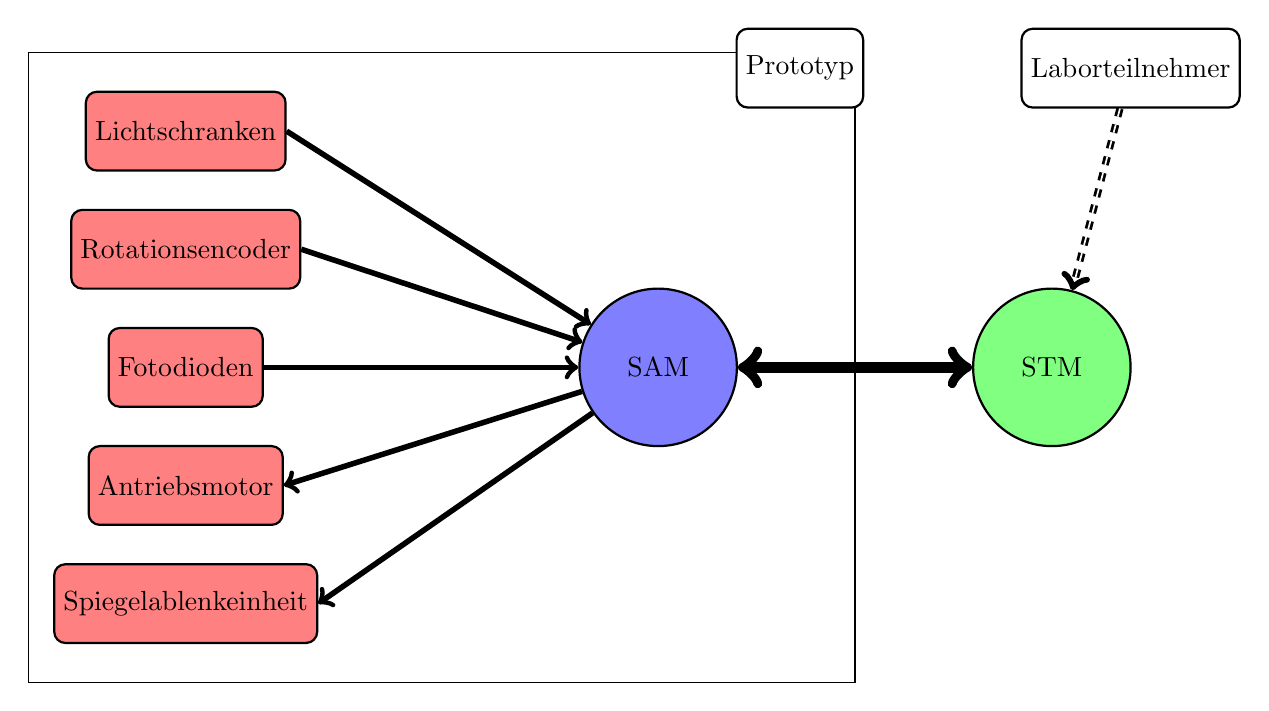
\begin{tikzpicture}[
every node/.style={draw, minimum size=1cm, thick, fill=white, rounded corners},
sam/.style={circle, minimum size=2cm, fill=blue!50},
stm/.style={circle, minimum size=2cm, fill=green!50},
sen/.style={fill=red!50}
]
\node[sam] at (6,0) (sam) {SAM};
\node[stm] at (11,0) (stm) {STM};
\node at (12,3.8) (tln) {Laborteilnehmer};
\node[sen] at (0,3) (li) {Lichtschranken};
\node[sen] at (0,1.5) (ro) {Rotationsencoder};
\node[sen] at (0,0) (fo) {Fotodioden};
\node[sen] at (0,-1.5) (an) {Antriebsmotor};
\node[sen] at (0,-3) (sp) {Spiegelablenkeinheit};

\draw[<->,line width=4pt] (sam) -- (stm);
\draw[<-,line width=2pt] (sam) -- (li.east);
\draw[<-,line width=2pt] (sam) -- (ro.east);
\draw[<-,line width=2pt] (sam) -- (fo.east);
\draw[->,line width=2pt] (sam) -- (an.east);
\draw[->,line width=2pt] (sam) -- (sp.east);
\draw[->,line width=1pt,dashed,double] (tln) -- (stm);

\draw (-2,-4) -- (-2,4) -- (8.5,4) -- (8.5,-4) -- (-2,-4);
\node at (7.8,3.8) (prot) {Prototyp};


\end{tikzpicture}
